\documentclass[english,aspectratio=169,14pt]{beamer}
\usepackage[utf8]{inputenc}
\usepackage{hyperref}
\usepackage{listings}

\usetheme{Madrid}
\useoutertheme{miniframes} % Alternatively: miniframes, infolines, split
\useinnertheme{circles}

\definecolor{CSUblue}{HTML}{002855} % CSU Blue (primary)
\definecolor{CSUgold}{HTML}{A89968} % CSU Gold (primary)

\usecolortheme[named=white]{structure} % albatross
\setbeamercolor{title}{fg=CSUblue}
\setbeamercolor{titlelike}{fg=white}
\setbeamercolor{frametitle}{fg=CSUblue}
\setbeamercolor{normal text}{bg=CSUblue,fg=white}

\AtBeginSection[]
{
  \begin{frame}
    \frametitle{Table of Contents}
    \tableofcontents[currentsection]
  \end{frame}
}

\logo{
\includegraphics[width=2cm]{images/logo}}

\lstset{
    %backgroundcolor=\color{black},
    %escapeinside={\%*}{*)},          % if you want to add LaTeX within your code
    language={[LaTeX]TeX},
    linewidth=0.8\linewidth,
    breaklines=true,
	tabsize=4,
	numbers=left,
	frame=single,
	showspaces=false,
	showtabs=false,
	upquote=true,
	showstringspaces=false,
	breakatwhitespace=true,
	escapeinside={(*@}{@*)},
	morekeywords={partial, var, value, get, set},
	%commentstyle=\fontfamily{\sfdefault}\color{comments}\itshape,
	%keywordstyle=\color{CSUgold}\textbf,
	%basicstyle=\ttfamily\small,
	%Colors
	numberstyle=\color{CSUgold},
	emphstyle={\color{operator}\bfseries},
	xleftmargin=1cm,
    backgroundcolor=\color{black},
    basicstyle=\color{CSUgold}\ttfamily\footnotesize,
    keywordstyle=\color{cyan},
    commentstyle=\color{gray},
    stringstyle=\color{blue},
    %numberstyle=\color{sviolet},
    identifierstyle=\color{white},
}


\title{Learn \LaTeX}
\author{Dr. Sean T. Hayes }
\date{April 8, 2020}
\institute[CSU]{Charleston Southern University}

\begin{document}

\begin{frame}
    \maketitle
\end{frame}

\section{\LaTeX{} Overview}

\begin{frame}{What is \LaTeX{}?}
    \begin{itemize}
        \item A document preparation system.
        \item Writers write in plain text (i.e., the source code)
        \item Markup tags define the document structure, stylize text (e.g., bold, italics), add citations, etc.
        \item The source document is compiled to an output file (e.g., PDF or DVI) suitable for printing or digital distribution.
    \end{itemize}
\end{frame}

\begin{frame}{Why use \LaTeX{}?}
    \begin{itemize}
        \item<1-> Clear separation the \emph{content} from the \emph{format} (using templates).

        \item<2-> High quality typography
        \begin{enumerate}
            \item Looks really sharp automatically (typography is an art)
            \item Easily create complex math formulas or use non-Latin characters.
            \item Endless customization of documents is possible, and also automatable.
        \end{enumerate}

        \item<3-> Dependable
        \begin{enumerate}
            \item Very stable, regardless of complexity.
            \item Free and Open Source
            \item Cross Platform and Backwards Compatible
        \end{enumerate}

        \item<4-> Plain-text source.
        \begin{enumerate}
            \item Viruses cannot ``hiding'' in the document.
            \item Works well with version control (e.g., git).
        \end{enumerate}
    \end{itemize}
\end{frame}

\begin{frame}{The challenges of learning \LaTeX}
    \begin{itemize}
        \item The learning curve may be steep.
        \item Syntax errors are common (like a programming language).
    \end{itemize}
\end{frame}

\section{Brief History}

\begin{frame}{Brief History: \TeX}
    \begin{columns}[T] % contents are top vertically aligned
    \begin{column}{9cm} % each column can also be its own environment
    Donald Knuth authored \emph{The Art of Programming}.
    \begin{enumerate}
        \item 1968, the first edition of the first volume was printed using mechanical (ink press onto paper).
        \item 1976, second edition printed using phototypesetting (inferior presentation)
        \item 1989, \TeX{} was released.
    \end{enumerate}

    \end{column}
    \begin{column}{5cm} % alternative top-align that's better for graphics

        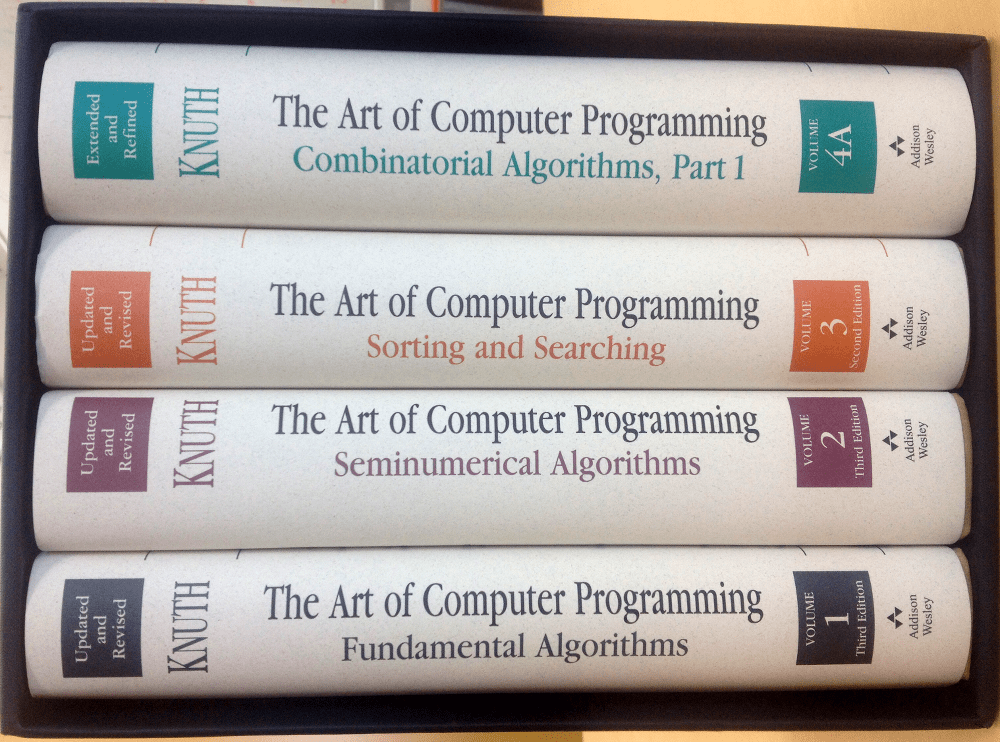
\includegraphics[width=\textwidth]{images/TheArtOfProgrammingBoxSet}
    \end{column}
    \end{columns}
\end{frame}

\begin{frame}{Brief History: \LaTeX}
    \begin{columns}[T] % contents are top vertically aligned
    \begin{column}{11cm} % each column can also be its own environment
    \begin{enumerate}
        \item 1984, Leslie Lamport created a set of macros for \TeX{} to simplify the typesetting, especially mathematical formulae.
        \item 1994, Released \LaTeXe, current version
        \item \LaTeX3 has been under development since the early 1990's with planned features for improved syntax, hyperlink support, arbitrary font access, and new documentation (see \href{https://github.com/latex3/latex3}{GitHub repo}).
    \end{enumerate}{}

    \end{column}
    \begin{column}{3cm}
        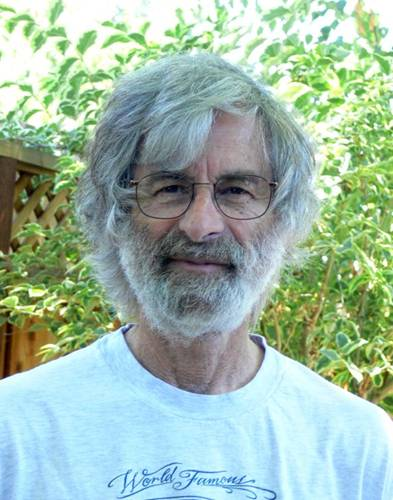
\includegraphics[width=\textwidth]{images/Leslie_Lamport}
    \end{column}
    \end{columns}
\end{frame}

\section{\LaTeX{} Syntax Basics}
\begin{frame}[t,fragile]{Writing your first piece of \LaTeX}
\begin{lstlisting}
\documentclass{article}
\begin{document}
   Hello world!

   This will be paragraph two.
\end{document}
\end{lstlisting}
\end{frame}

\begin{frame}[t,fragile]{Add your name and title}
\begin{lstlisting}
\documentclass{article}

% This is the preamble
\title{Title Here}
\author{Name Here}
\date{\today}
\begin{document}
    \maketitle
    Hello world!

    This will be paragraph two.
\end{document}
\end{lstlisting}
\end{frame}

\begin{frame}{Resources}
    \begin{enumerate}
        \item \url{https://en.wikibooks.org/wiki/LaTeX}
        \item \url{https://ctan.org/} \\
        \url{https://www.acm.org/publications/proceedings-template}
        \item \url{https://github.com/DoctorHayes/learn-latex-presentation}
    \end{enumerate}{}


\end{frame}

\end{document}
